\newpage
\section{Εισαγωγή}
Η επιστήμη των δεδομένων (\textlatin{Data science}) είναι
μια επιστήμη που αφορά την εξαγωγή γνώσης από δεδομένα
(δομημένα ή αδόμητα) και για να το πετύχει αυτό συνδυάζει
γνώσεις από διάφορες άλλες επιστήμες όπως:
\begin{itemize}
    \item Μαθηματικά
    \item Στατιστική
    \item Προγραμματισμός
    \item Προγνωστική ανάλυση (\textlatin{Predictive analysis})
    \item Εξόρυξη δεδομένων (\textlatin{Data mining})
    \item Τεχνητή Νοημοσύνη (\textlatin{Artificial intelligence})
    \item Μηχανική μάθηση (\textlatin{Machine learning})
\end{itemize}
Επιπλέον, η επιστήμη των δεδομένων συνδυάζει τα παραπάνω με
τη γνώση κάποιου ειδικού τομέα (όπως η ιατρική) με σκοπό να
δώσει λύση σε ένα συγκεκριμένο πρόβλημα \cite{wikiDS}
\begin{figure}[H]
    \centering
    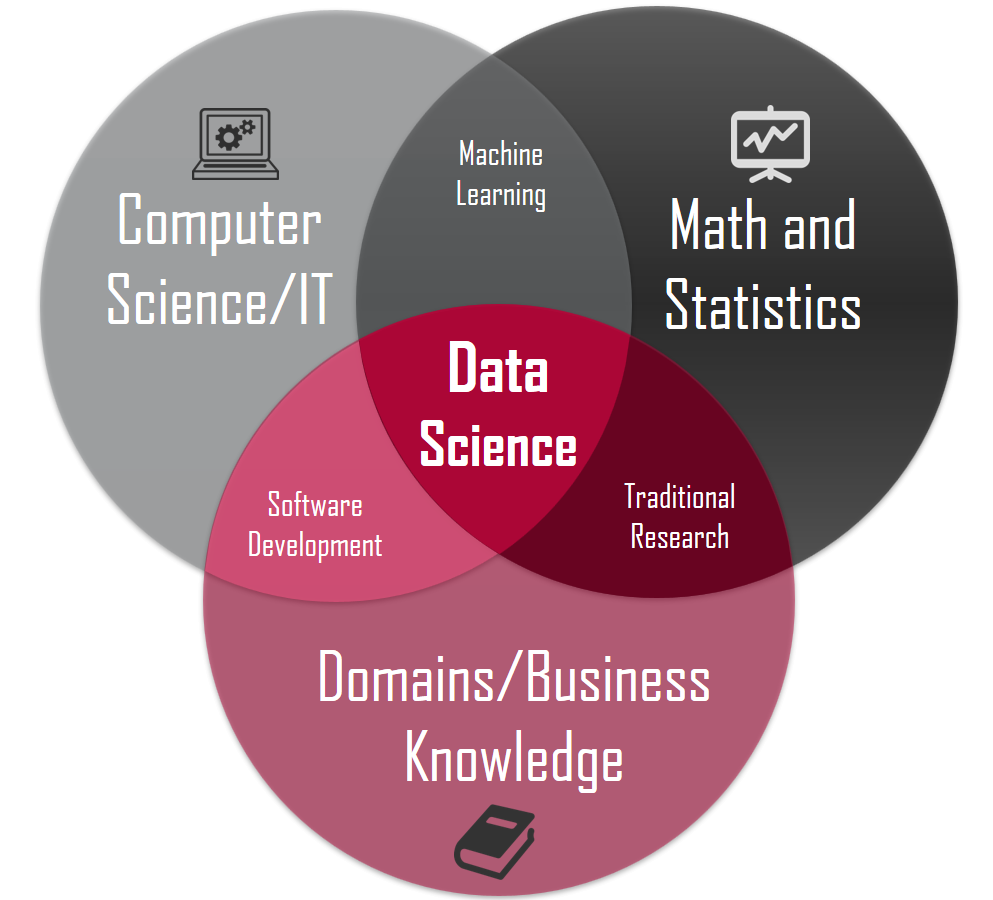
\includegraphics[width=0.4\textwidth]{images/dataScienceKnowledge.png}
    \caption{Γνώσεις που συνδυάζει η επιστήμη των δεδομένων}
\end{figure}

Σε αυτή την εργασία θα ασχοληθούμε κυρίως με την τεχνητή
νοημοσύνη και τη μηχανική μάθηση και πιο συγκεκριμένα με τους
αλγόριθμους που εφαρμόζονται στην επιστήμη των δεδομένων.
Θα δοθεί αναλυτική εξήγηση για πολλούς χρήσιμους αλγόριθμους
και θα υλοποιηθούν οι πιο σημαντικοί από αυτούς με τη χρήση
της γλώσσας προγραμματισμού \textlatin{C++} η οποία θα μας δώσει τη
δυνατότητα να φτιάξουμε γρήγορα προγράμματα.

Οι αλγόριθμοι που θα εξετάσουμε μπορούν να χωριστούν σε πέντε
ομάδες με βάση τη χρήση τους και αυτές είναι:
\begin{itemize}
    \item Αλγόριθμοι ταξινόμησής (\textlatin{Classification})
    \item Αλγόριθμοι παλινδρόμησης (\textlatin{Regression})
    \item Αλγόριθμοι ομαδοποίησης (\textlatin{Clustering})
    \item Αλγόριθμοι μείωσης διαστάσεων (\textlatin{Dimentionality reduction})
    \item Αλγόριθμοι ενισχυτικής μάθησης (\textlatin{Reinforcement learning})
    \item Αλγόριθμοι ανίχνευσης ανωμαλίας (\textlatin{Anomaly detection})
\end{itemize}
Μας ενδιαφέρουν ιδιαίτερα οι πρώτες τρεις ομάδες
καθώς είναι αυτές που
εμφανίζονται πιο συχνά.Οι παλινδρομητές και οι ταξινομητές είναι πολύ παρόμοιοι αλγόριθμοι οι οποίοι ανήκουν στους αλγόριθμους εποπτευόμενης
μάθησης (\textlatin{Supervised learning}) και χρησιμοποιούνται
για να κάνουν προβλέψεις σύμφωνα με τα δεδομένα
που τους έχουμε
δώσει. Η διαφορά τους είναι ότι η ταξινόμηση προσπαθεί να
προβλέψει την κλάση των καινούριων δεδομένων και να τα
κατηγοριοποιήσει σύμφωνα με τις υπάρχουσες κατηγορίες, ενώ η
παλινδρόμηση προσπαθεί να προβλέψει την τιμή κάποιου στοιχείου
για τα καινούρια δεδομένα σύμφωνα με μια συνάρτηση που
έφτιαξε
από τα υπάρχοντα δεδομένα. Οι περισσότεροι αλγόριθμοι ταξινόμησης είναι και
αλγόριθμοι παλινδρόμησης και το αντίστροφο. Από την άλλη οι αλγόριθμοι
ομαδοποίησης είναι μη εποπτευόμενης μάθησης και χρησιμοποιούνται σε αδόμητα
δεδομένα για να τα χωρίσουν σε ομάδες.
\begin{figure}[H]
    \centering
    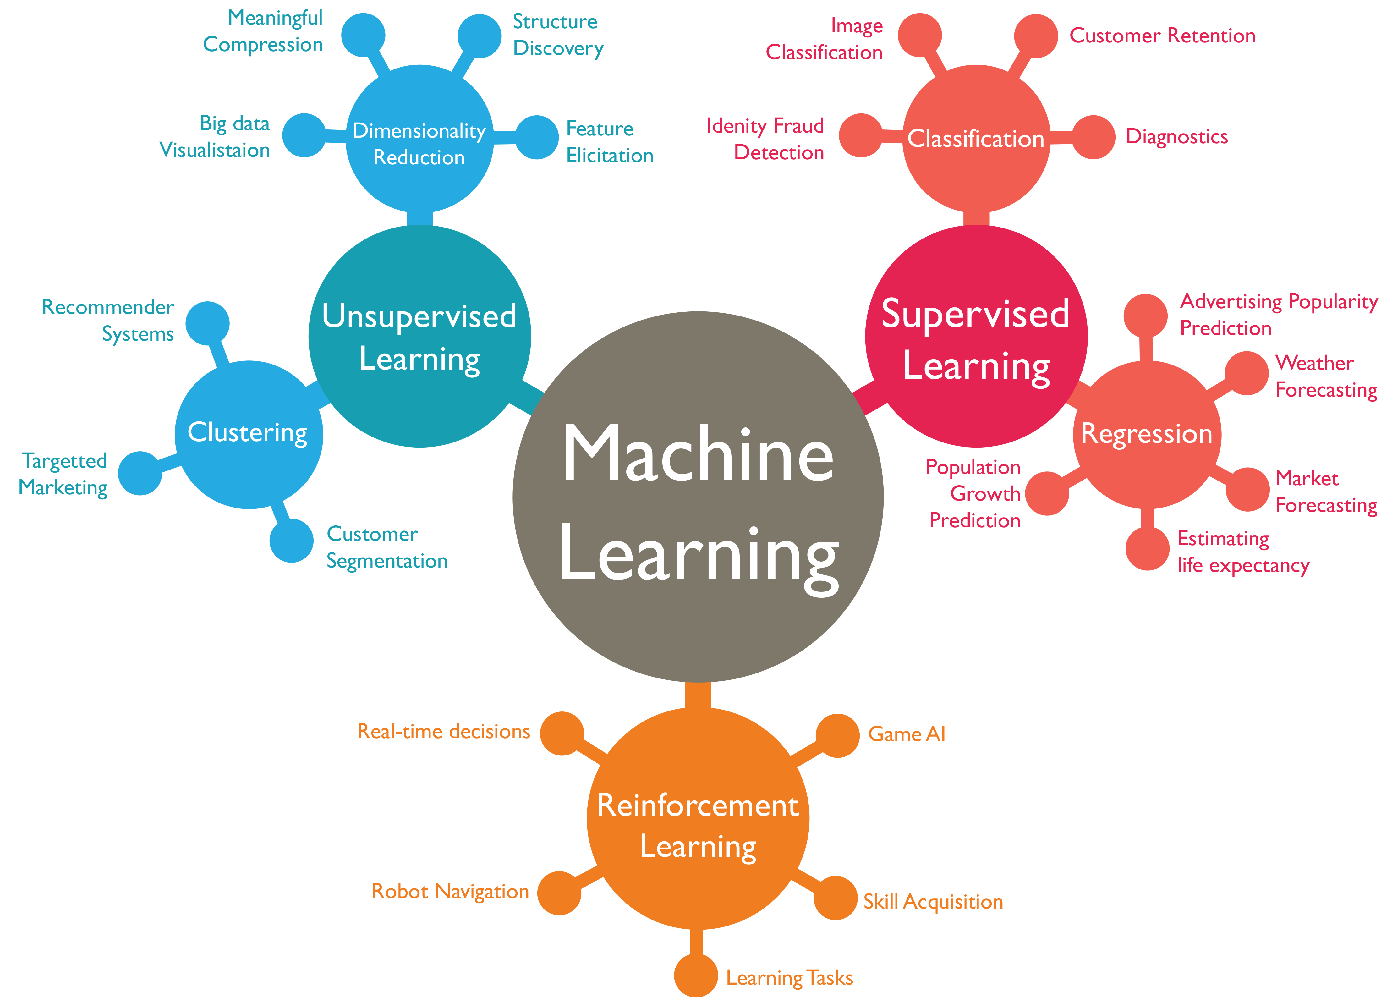
\includegraphics[width=0.7\textwidth]{images/machineLearning.png}
    \caption{Αλγόριθμοι μηχανικής μάθησης}
\end{figure}